\chapter{21/09/16 - Introduzione, parte seconda}
\section{Breve descrizione della lezione}
Da scrivere.
\section{Curve algebriche non singolari}

Introduciamo anzitutto il concetto di singolarità.

\notamargine{Il contesto in cui ci troviamo è $\bbP_n(\bbK)$, dove $\bbK$ è un campo che spesso sarà $\bbC$ e $n$ spesso sarà 2.}
Data una curva $\gamma$ descritta come zeri in $\bbP_n(\bbK)$ di $f \in \bbK[x_0, \ldots,x_n]$ omogenea, diciamo che un punto è 
\smallcaps{singolare} se, in un senso che renderemo più preciso, non esiste una sola retta tangente alla curva passante per il punto. 

\newthought{Geometricamente}, un punto $p \in \gamma$ è singolare se esiste più di una retta $r$ passante per $p$ con ordine di contatto $\geq 2$. \notamargine{L'ordine di contatto di $r$ con $\gamma$ in $p$ è la molteplicità di $p$ come zero del sistema $r=0,f=0$.}
\vspace{1em}

%%mettere un disegno con cuspide e nodo
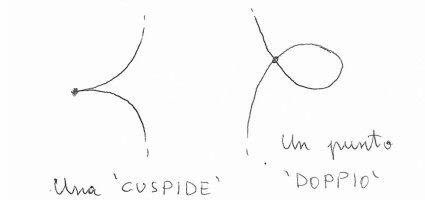
\includegraphics[width=20em]{punti-singolari.jpeg}

\newthought{Algebricamente}, un punto $p$ zero di $f$ è singolare se $\de{x_i}f(p)=0$ per $i=0,\ldots,n$ (ha il differenziale nullo). 
\notamargine{Se il campo ha caratteristica 0, notare che $\de{x_i}f(p) = 0$ per ogni $i$ implica $f(p)=0$ per il \href{https://it.wikipedia.org/wiki/Funzione_omogenea}{teorema di eulero} sulle funzioni omogenee.}



\section{Cubiche, forma di Weierstrass}
Nel caso speciale di $n=2$, $\chr \bbK =0$ c'è un importante risultato di classificazione delle curve non singolari. 
\notamargine{Una curva si dice non singolare se ogni suo punto è non singolare.} 

Consideriamo curve descritte da
$$ zy^2= ax^3+bx^2z+cxz^2+dz^3 $$
 dove $ax^3+bx^2+cx+d$ è un polinomio senza radici multiple, detta \smallcaps{forma di weierstrass}. Allora è non singolare. Imponiamo infatti le tre equazioni:

%% ESERCIZIO: dimostrare che la forma di weierstrass è non singolare

$$ \left\{ 
\begin{matrix}
&3ax^2&+2bxz&+cz^2 & = & -\de{x}f & = 0 \\
&&yz& & = & \de{y}f / 2 &= 0 \\
y^2 &-bx^2&-2cx&-3dz^2 & = & \de{z}f& = 0 \\
ax^3&+bx^2z&+cxz^2&+dz^3& = & zy^2&
\end{matrix}
\right.$$

Dalla (2) abbiamo due casi:

\begin{itemize}
	\item Se $z=0$ allora (4) dà $x=0$ e dunque $y=0$ dalla (3), assurdo.
	\notamargine{ Siamo nel proiettivo: $x=y=z=0$ non è un punto!} 

	\item Se $y = 0$, $z \neq 0$ allora (4) dà $q(x/z) = 0$ e (1) dà $q'(x/z) = 0$ (dove $q$ è il polinomio di coefficienti $a,b,c,d$). Ma allora $x/z$ sarebbe una radice multipla di $q$, assurdo.  
	\notamargine{Infatti se $\chr \bbK = 0$ vale il criterio della derivata.}
\end{itemize}

Viceversa, data una curva cubica non singolare, può essere descritta da un polinomio in forma di weierstrass. Algebricamente, per ogni polinomio omogeneo $f$ di grado 3 con differenziale mai nullo, esiste una $L \in \bbP GL_2(\bbK) $ tale che $f \circ L$ (che è ancora un polinomio omogeneo di grado 3) è in forma di weierstrass. 
\paragraph{IDEA}. Si dimostra che esiste un punto di flesso (?), e poi si considera una proiettività che scambia il  punto di flesso con il punto all'infinito. A quel punto, con pochi conti, si arriva alla forma di weierstrass.

\section{Cubiche, struttura di gruppo}

Sia $\bbK$ algebricamente chiuso. Osserviamo che presi due punti $P,Q$ su una cubica $\gamma$ e tracciata la retta $r$ per $P,Q$, essa interseca $\gamma$ esattamente in un altro punto $R:=P * Q = Q*P$. \notamargine{Vedi il \href{https://en.wikipedia.org/wiki/B\%C3\%A9zout's_theorem}{Teorema di Bezòut}.}

Fissata un'origine $O \in \gamma$, si può dimostrare che l'operazione $(P,Q) \mapsto P \cdot Q = O*(P*Q)$ rende $\gamma$ un gruppo (banalmente) abeliano. Il cambio dell'origine dà luogo a un gruppo isomorfo. Infatti se $O,O'$ sono due origini diverse, detto $O'' = O*O'$, la mappa $P \mapsto O'' * P$ è l'isomorfismo cercato:
\notamargine{Solitamente, nella forma di weierstrass, si prende $O=(0:1:0)$, il punto all'infinito.}
$$ O'' * (P \cdot' Q) = O'' * O'*P*Q = O*P*Q $$
$$ (O''*P) \cdot (O''*Q) = (O*O'')*(P*O'')*Q = O'*O''*P*Q=O*P*Q$$

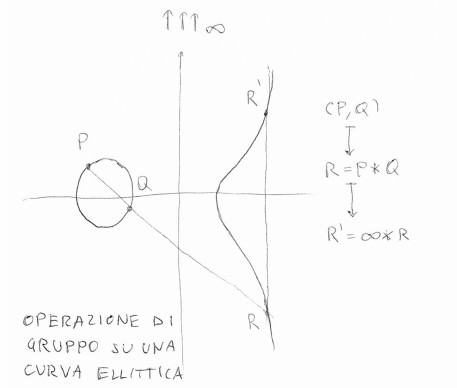
\includegraphics[width=16em]{gruppo-cubica.jpeg}

L'associatività è la proprietà più impegnativa da dimostrare. Vale la pena di notare che l'operazione è una funzione razionale delle coordinate dei punti. 
\section{Funzioni ellittiche, reticoli}

\section{Moduli}

\section{Superfici di Riemann}
\notamargine{Per quanto possa sembrare strano, è vero}

